\subsection{Model-to-Model Transformation: from OpenAPI to CPN}
\label{sec:transformation}

According to~\cite{vanderAalst2016}, depending on the input data and the questions that need to be addressed, an appropriate model and abstraction level must be chosen. In this paper, we consider that CPN provides a suitable abstraction and model to represent REST APIs because: (i) control flow and data flow need to be modeled together; (ii) the literature shows that REST APIs can be modeled as CPNs~\cite{decker2008restful, li2011design, li2015designing}; and (iii) there are conformance checking algorithms for CPN~\cite{carrasquel2020checking}. Below, we present a model transformation from a valid OpenAPI document to a CPN and illustrate it with the following running example.

%
%
Algorithm~\ref{lst:algorithm} describes the steps for the model transformation. As an input, it needs an OpenAPI specification {\tt doc}. As an output, it generates a Colored PetriNet $\mathcal{C}=\tuple{P,T,A,V,G,E,\pi}$ that represents {\tt doc}. %In the algorithm, names defined in Snake Case (like http\_method, create\_transition, etc) are names of variables and methods created by the algorithm, while names in Camel Case and Pascal Case (like PathItemObject, ResponseObject, responses, etc) are names of objects and structures of the OpenAPI Specification.


\begin{algorithm}
\KwIn{An OpenAPI specification {\tt doc}.}
\KwOut{A Colored Petri net $\mathcal{C}=\tuple{P,T,A,V,G,E,\pi}$.}

\tcc{Create all the transitions related to paths}
$\mathcal{C}$ = createTransitionsForPaths({\tt doc}) (see Algorithm~\ref{lst:algorithm_transitions})\;

\tcc{Connect transitions related to paths}
$\mathcal{C}$ = connectTransitionsForPaths({\tt doc}, $\mathcal{C}$) (see Algorithm~\ref{lst:algorithm_connect_transitions})\;

Remove disconnected transitions and places in $\mathcal{C}$\;
\Return  $\mathcal{C}$\;

\caption{Creation of a CPN from an OpenAPI specification.}
\label{lst:algorithm}
\end{algorithm}


\begin{algorithm}
\KwIn{An OpenAPI specification {\tt doc}.}
\KwOut{A Colored Petri net $\mathcal{C}=\tuple{P,T,A,V,G,E,\pi}$.}

Create an empty CPN $\mathcal{C}=\tuple{P,T,A,V,G,E,\pi}$\;
\ForEach{{\tt path} $\mathcal{P} \in$ {\tt doc}}{
	\ForEach{{\tt operation} $\mathcal{O} \in \mathcal{P}$ }{
		{\tt operationId}  $\leftarrow$ Get {\tt operationId} from $\mathcal{O}$\;
		{\tt HTTPMethod} $\leftarrow$ Get {\tt HTTPmethod} from $\mathcal{O}$\;
		\ForEach{{\tt response} $\mathcal{R} \in \mathcal{O}$ }{
			{\tt HTTPStatusCode} $\leftarrow$ Get {\tt HTTP-status-code} from $\mathcal{R}$\;
			Create a transition $t$, tagging it as {\tt HTTPMethod-path-HTTPStatusCode} and with id {\tt operationId}\;
			Add transition $t$ to $\mathcal{C}$ (i.e., $T=T \cup \{t\}$)\;
			Create a place $p=\preset{t}$\;
			Add place $p$ to $\mathcal{C}$ (i.e., $P=P \cup \{p\}$)\;
		}
		\If{$\exists$ {\tt parameters $\mathcal{U}$} $\in \mathcal{O}$}{
				{\tt paramName}   $\leftarrow$ Get {\tt name} from $\mathcal{U}$\;
				Label the output arc of $p$ as {\tt paramName}\;
		}
	}	
}
\Return  $\mathcal{C}$
\caption{Creation of CPN transitions representing paths in an OpenAPI specification.}
\label{lst:algorithm_transitions}
\end{algorithm}

\begin{algorithm}
\KwIn{An OpenAPI specification {\tt doc} and a Colored Petri net $\mathcal{C}=\tuple{P,T,A,V,G,E,\pi}$.}
\KwOut{An updated Colored Petri net $\mathcal{C}=\tuple{P,T,A,V,G,E,\pi}$.}

\ForEach{{\tt path} $\mathcal{P} \in$ {\tt doc}}{
	\ForEach{{\tt operation} $\mathcal{O} \in \mathcal{P}$ }{
		{\tt operationId}  $\leftarrow$ Get {\tt operationId} from $\mathcal{O}$\;
		{\tt HTTPMethod} $\leftarrow$ Get {\tt HTTPmethod} from $\mathcal{O}$\;
		\ForEach{{\tt response} $\mathcal{R} \in \mathcal{O}$ }{
			Let $t \in \mathcal{T}$ be the transition with id {\tt operationId}\;
			\If{$\exists$ {\tt links} $\mathcal{L}$ $\in \mathcal{R}$}{
				{\tt operationId}$^\prime$  $\leftarrow$ Get {\tt operationId} from $\mathcal{L}$\;
				{\tt parameter}  $\leftarrow$ Get {\tt parameters} from $\mathcal{L}$\;
				Let $t^\prime \in \mathcal{T}$ be the transition with id {\tt operationId}$^\prime$\;
				Create an arc connecting $\postset{t}=\preset{t^\prime}$\;
				Label the input arc of $\postset{t}$ with 	{\tt parameter} \;
			}
		}
	}	
}

\Return  $\mathcal{C}$
\caption{Connection of CPN transitions representing paths in an OpenAPI specification.}
\label{lst:algorithm_connect_transitions}
\end{algorithm}



First, we create all the transitions related to paths in the OpenAPI specification, as indicated by Algorithm~\ref{lst:algorithm_transitions}. Basically, this algorithm iterates over the paths and for each operation on the path, it iterates over the responses (lines 6--17), creating a new transition $t$ that represents such a response (line 8). The {\tt operationId} and {\tt HTTPMethod} of an operation, as well as its {\tt HTTPStatusCode}, are taken as variables to make up the tagging of $t$. For each transition $t$, we also create a preset place $p=\preset{t}$. Also, the arc connecting $p$ and $t$ is labeled by the name of the operation parameter (if any).
% 
The second part of the algorithm is related to the connection of path-related transitions (see Algorithm~\ref{lst:algorithm_connect_transitions}). We iterate over the paths and for operation on the path, we iterate over the responses (lines 5--14 of Algorithm~\ref{lst:algorithm_connect_transitions}). Each response is analyzed and if it is linked to any other path, the transitions representing both paths are connected via the preset place of the transitions that represents the target path.
% 
Finally, we remove all transitions that do not have connections to places (line $5$ of Algorithm~\ref{lst:algorithm}), and we return the updated CPN (line $6$).

Applying Algorithm~\ref{lst:algorithm} to the OpenAPI specification shown in~\ref{apx:openapi_example}, we will obtain a CPN as the one depicted in Figure~\ref{fig:running_example_transformation}. Note that the transition ``{\tt \path{post-/rest/user/login/-200}}'' is created by the path {\tt \path{/rest/user/login}}, the operation {\tt post}, and the response code 200. Similarly,  the transition ``{\tt \path{get-/rest/user/\{bid\}/-200}}'' is created by the path {\tt /rest/basket/\{bid\}}, the operation {\tt get}, and the response code 200. The preset arc is labeled with {\tt bid}, given the {\tt parameter name} of the operation. Finally,  both transitions are joined as the response of the path {\tt /rest/user/login} is linked to {\tt getBasketById}, which is represented by the transition {\tt \path{get-/rest/user/\{bid\}/-200}}.

\begin{figure}
    \center
    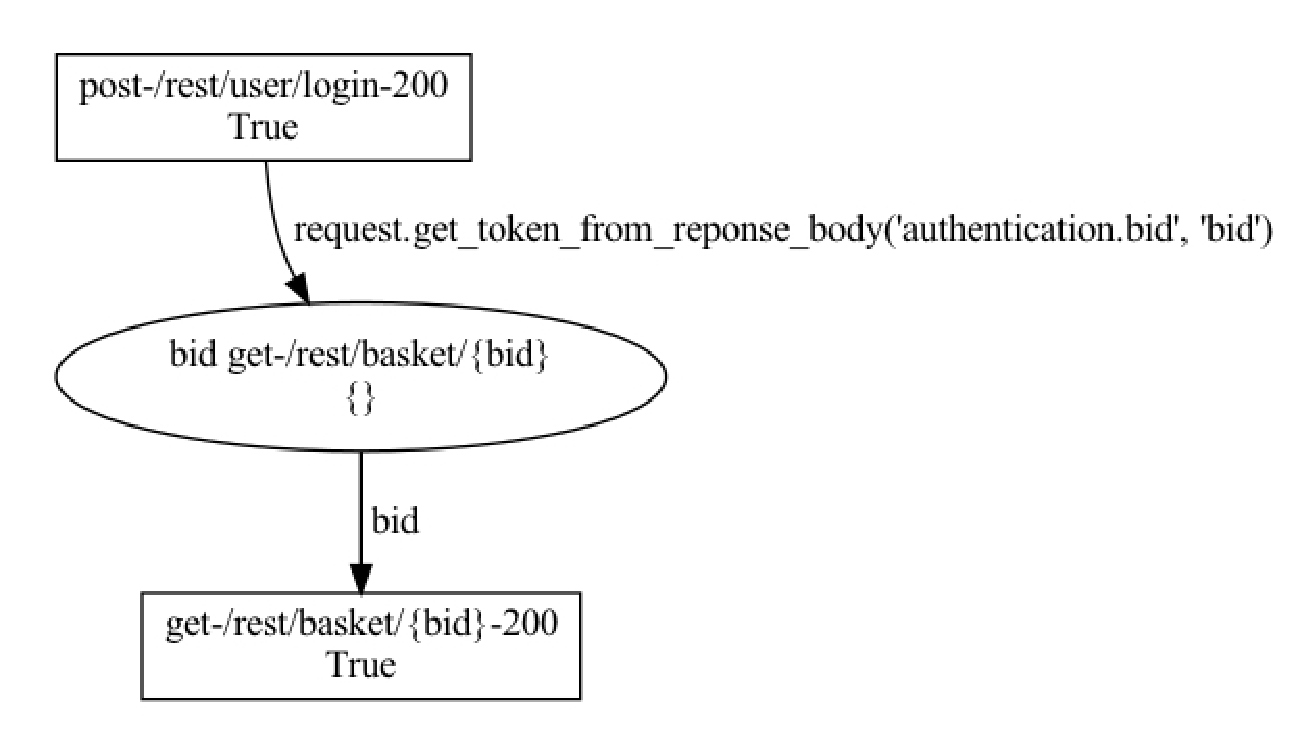
\includegraphics[width=1\columnwidth]{figures/SimpleJuiceShop-initial-state}
    \caption{Transformation from OpenAPI specification to CPN.}
    \label{fig:running_example_transformation}
\end{figure}


To show the generality of our transformation approach, we apply Algorithm~\ref{lst:algorithm} to a more complex example. In particular, we consider the  lightweight open-source note-taking service called {\tt Memos}\footnote{Accessible in \url{https://github.com/usememos/memos}}. The API of {\tt Memos} had a BOLA vulnerability related to note archiving operation that was found and fixed in 2022~\cite{huntr2022}. Figure~\ref{fig:memos_inital_state} shows the CPN obtained after the automatic transformation from {\tt Memos} OpenAPI specification to CPN performed by our algorithm. Let us remark that before applying the transformation we have slightly modified the original source code to recreate the vulnerability\footnote{The vulnerable source code is accessible in \url{https://github.com/ailton07/memos-with-BOLA/blob/main/api/v1/openapi.yaml}}.

Similar to the previous example, the transition \path{post-/api/v1/memo-200} is created by the path \path{/api/v1/memo}, the operation \path{post}, and the response code $200$. Likewise, the transition \path{get-/api/v1/memo-200} is created by the path \path{/api/v1/memo}, the operation \path{get}, and the response code $200$. Finally, transitions starting with \path{patch-/api/v1/memo/{memoId}} are created by the path \path{/api/v1/memo/{memoId}}, the operation \path{patch}, and the respective response code $200$, $400$, $401$, $404$, $500$. These three endpoints comprise the flows where the user can list their notes, create new notes, and archive their already created notes, respectively.

\begin{figure*}
    \center
    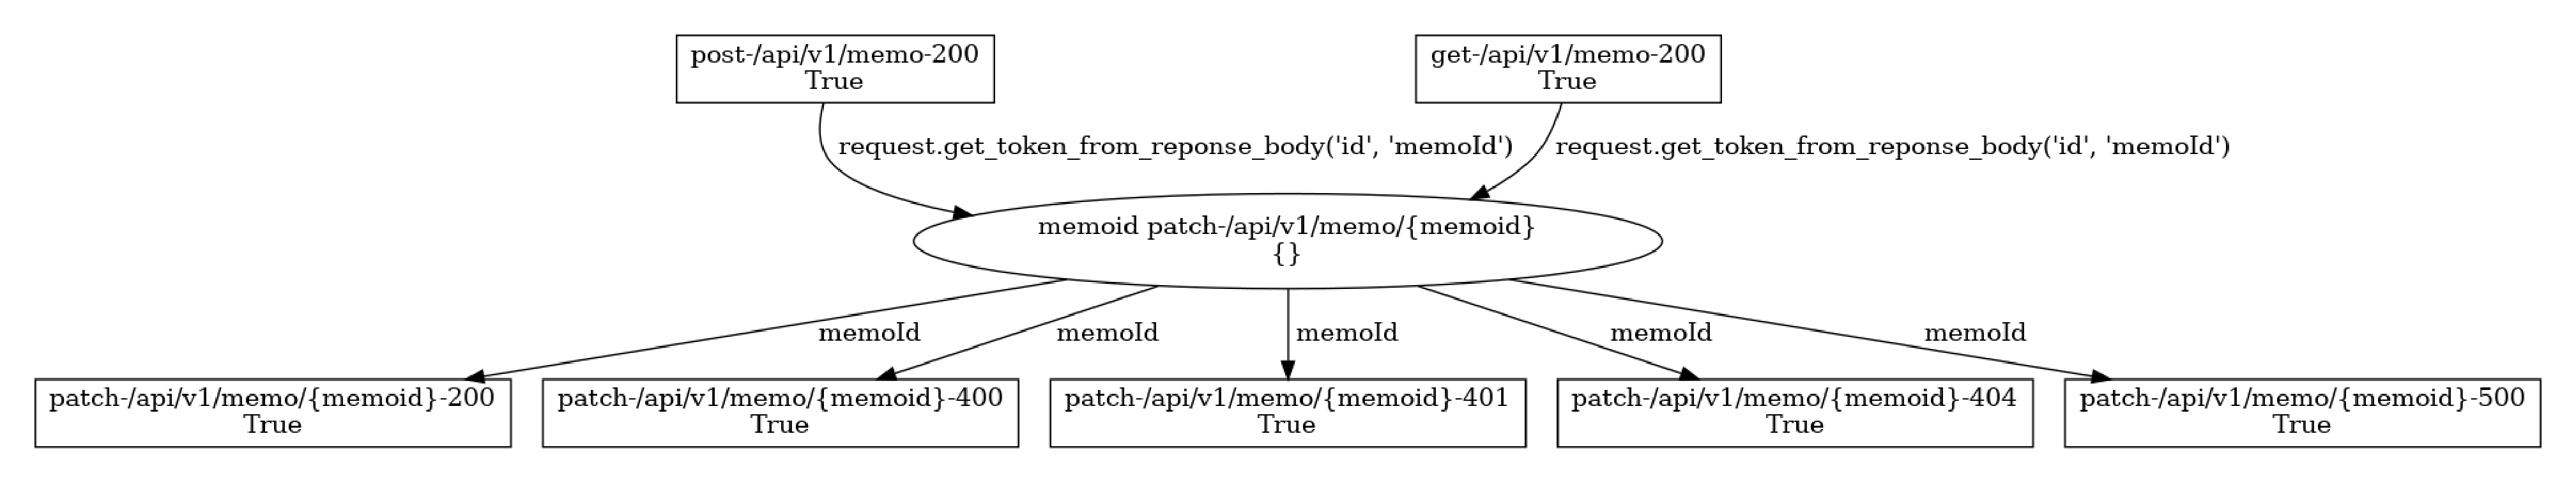
\includegraphics[width=2\columnwidth]{figures/memos-0-initial-state}
    \caption{Transformation from {\tt Memos} OpenAPI specification to CPN.}
    \label{fig:memos_inital_state}
\end{figure*}
